\newpage
\section{Spezifikation}
Basierend auf dem entwickelten Konzept und den definierten Anforderungen wird die detaillierte Spezifikation des Systems ausgearbeitet. Diese umfasst die Architektur des gesamten Systems, welche die Aufteilung in einzelne Komponenten und deren Interaktion untereinander beschreibt. Ebenso wurden die Schnittstellen zwischen den Komponenten definiert. Weiterhin wird erläutert, wie das System mit seiner Umgebung interagiert. Die technische Spezifikation umfasst die verwendete Hardware sowie die eingesetzten Protokolle und Standards, die für Umsetzung der einzelnen Komponenten benötigt werden. 

Zur besseren Veranschaulichung des Gesamtsystems, Beziehungen zwischen den Komponenten und der Abläufe wurden, wo sinnvoll, Diagramme erstellt. Diese visualisieren bestimmte Zusammenhänge. Bei der Erstellung dieser Diagramme wurde das SA/RT-Entwurfskonzept als Orientierungshilfe genutzt. Aufgrund der des hohen Umfangs bzw. der Komplexität des Projekts wurden die strengen Vorgaben des SA/RT-Konzepts jedoch flexibel gehandhabt und nicht strikt befolgt.

\subsection{Architektur}
Die Architektur des Projekts bietet eine Gesamtdarstellung des Systems und zeigt, wie die verschiedenen Komponenten miteinander interagieren. Das System gliedert sich in vier Hauptbereiche: Audioverarbeitung, Benutzeroberfläche (User Interface) und das neuronale Netz und das Dateimanagement.

\subsubsection{Systemkontext}

\textbf{I M A} interagiert als komplexes System mit zahlreichen Peripherien und externen Libraries. 

In Abbildung \ref{fig:context_diagram_gesamt} wird diese Interaktion durch ein Kontextdiagramm deutlich gemacht.

\begin{figure}[H]
   	\centering
   	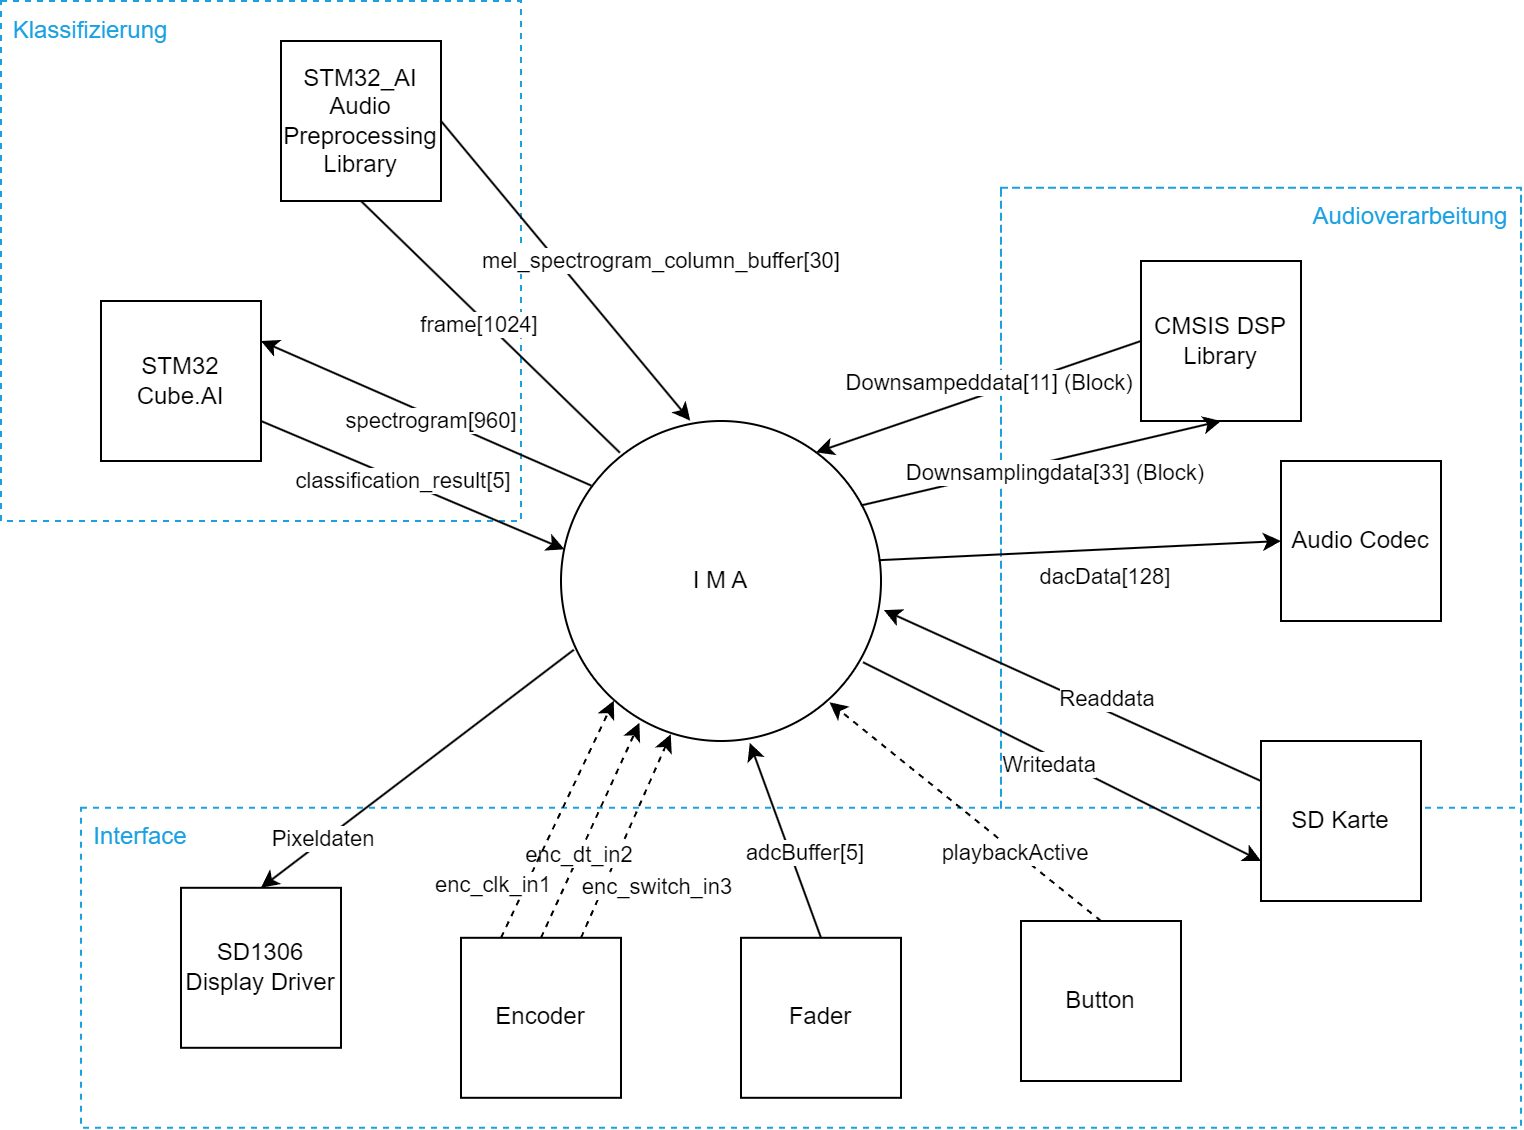
\includegraphics[width=0.8\textwidth]{images/04_spezifikation/kontextdiagramm_gesamt.drawio.png}
   	\caption{Kontextdiagramm des Gesamtsystems}
   	\label{fig:context_diagram_gesamt}
\end{figure}

\paragraph{Klassifizierung}

Die Klassifizierung durch das Neuronale Netz setzt die proprietäre \textbf{STM32.CubeAI} Umgebung voraus (näheres dazu im Abschnitt \ref{stm32-cube-ai}). Das neuronale Netz erhält als Eingabewert ein Spektrogramm mit 960 Reihen, und liefert daraufhin ein Klassifikationsergebnis mit den \hyperlink{nn-classes}{5 Klassen} zurück.

Da das Neuronale Netz die Klassifizierung über ein Spektrogramm, und nicht mit den rohen Audiosamples vollzieht, müssen die Audiodaten zunächst in ein solches Spektrogramm umgewandelt werden. Das geschieht Reihenweise, wie in Abschnitt \ref{sec:approach-audio-classification} beschrieben. Die Bibliothek für diese Umwandlung ist die ebenfalls proprietäre \textbf{STM32\_AI\_Audio\_Preprocessing\_Libray}. Der Input der Umwandlungsfunktion ist ein Buffer von 1024 Samples(\mintinline{c}|frame[1024]|). Der Rückgabewert ist eine Reihe des Spektrogramms (\mintinline{c}|mel_spectrogram_column_buffer[30]|).

\paragraph{Audioverarbeitung}

Um sicherzustellen, dass die \textbf{STM32\_AI\_Audio\_Preprocessing\_Libray} die zu klassifizierenden Audiodaten im richtigen Format erhält, müssen diese zuerst umgewandelt werden. Wie in Abschnitt \ref{sec:audio-downsampling} beschrieben, sind dafür Downsampling von 44.1kHz auf 16kHz Samplerate und die Umwandlung von Stereo auf Mono erforderlich. Für diese Schritte wird die Open-Source \textbf{CMSIS DSP Library} verwendet.

Bei der Audiowiedergabe erhält der Audio Codec pro Iteration den gesamten Audiobuffer \mintinline{c}|dacData[256]|.

\paragraph{Interface}

Um das Menü anzuzeigen, erhält der Treiber des Displays Strings, welche er intern in Pixeldaten umwandelt, sowie Linieninformationen in Form von Pixeldaten. 

Es sind 3 GPIO Inputs für die Nutzung des Encoders erforderlich. \mintinline{c}|enc_clk_in1| und \mintinline{c}|enc_dt_in2| sind für die Auswertung des Drehimpulsgebers nötig. \mintinline{c}|enc_switch_in3| dient für die Push-Button Funktion des Encoders.

Die 5 Fader werden über das Array \mintinline{c}|adcBuffer[5]| vom ADC über die DMA befüllt.

Der Play-Button schaltet das GPIO Signal \mintinline{c}|playbackActive|, womit die Audio Wiedergabe gestartet wird.

\paragraph{Dateimanagement}

Das \hyperlink{Dateisystem}{Dateimanagement} der Applikation wird über ein die C-Struktur \mintinline{c}|struct Filemanager| realisiert, das die Dateizugriffe auf die Audiodateien organisiert und die persistente Speicherung der Klassifizierungsdaten durchführt.  

Um die Klassifizierungsdaten zu speichern, wird eine neue Datei erstellt oder eine bestehende Datei geöffnet. Die Daten werden dann im ASCII- oder Binärformat in die Datei geschrieben. Der Filemanager-Struct verwaltet dabei die Datei-Handles und stellt sicher, dass die Datei nach dem Schreibvorgang ordnungsgemäß geschlossen wird.

\subsubsection{Zustandsautomat}

Zur detaillierten Darstellung des Funktionsablaufs und zur präzisen Planung des Zusammenspiels der Einzelkomponenten wurde ein Zustandsautomat entwickelt, der sich am SA/RT-Entwurfsmodell orientiert. 

Die Struktur und die Übergänge dieses Zustandsautomaten sind in Abbildung \ref{fig:fsm} veranschaulicht. Diese Abbildung bietet eine umfassende Visualisierung der verschiedenen Zustände und deren Wechselwirkungen innerhalb des Systems.

\begin{figure}[H]
   	\centering
   	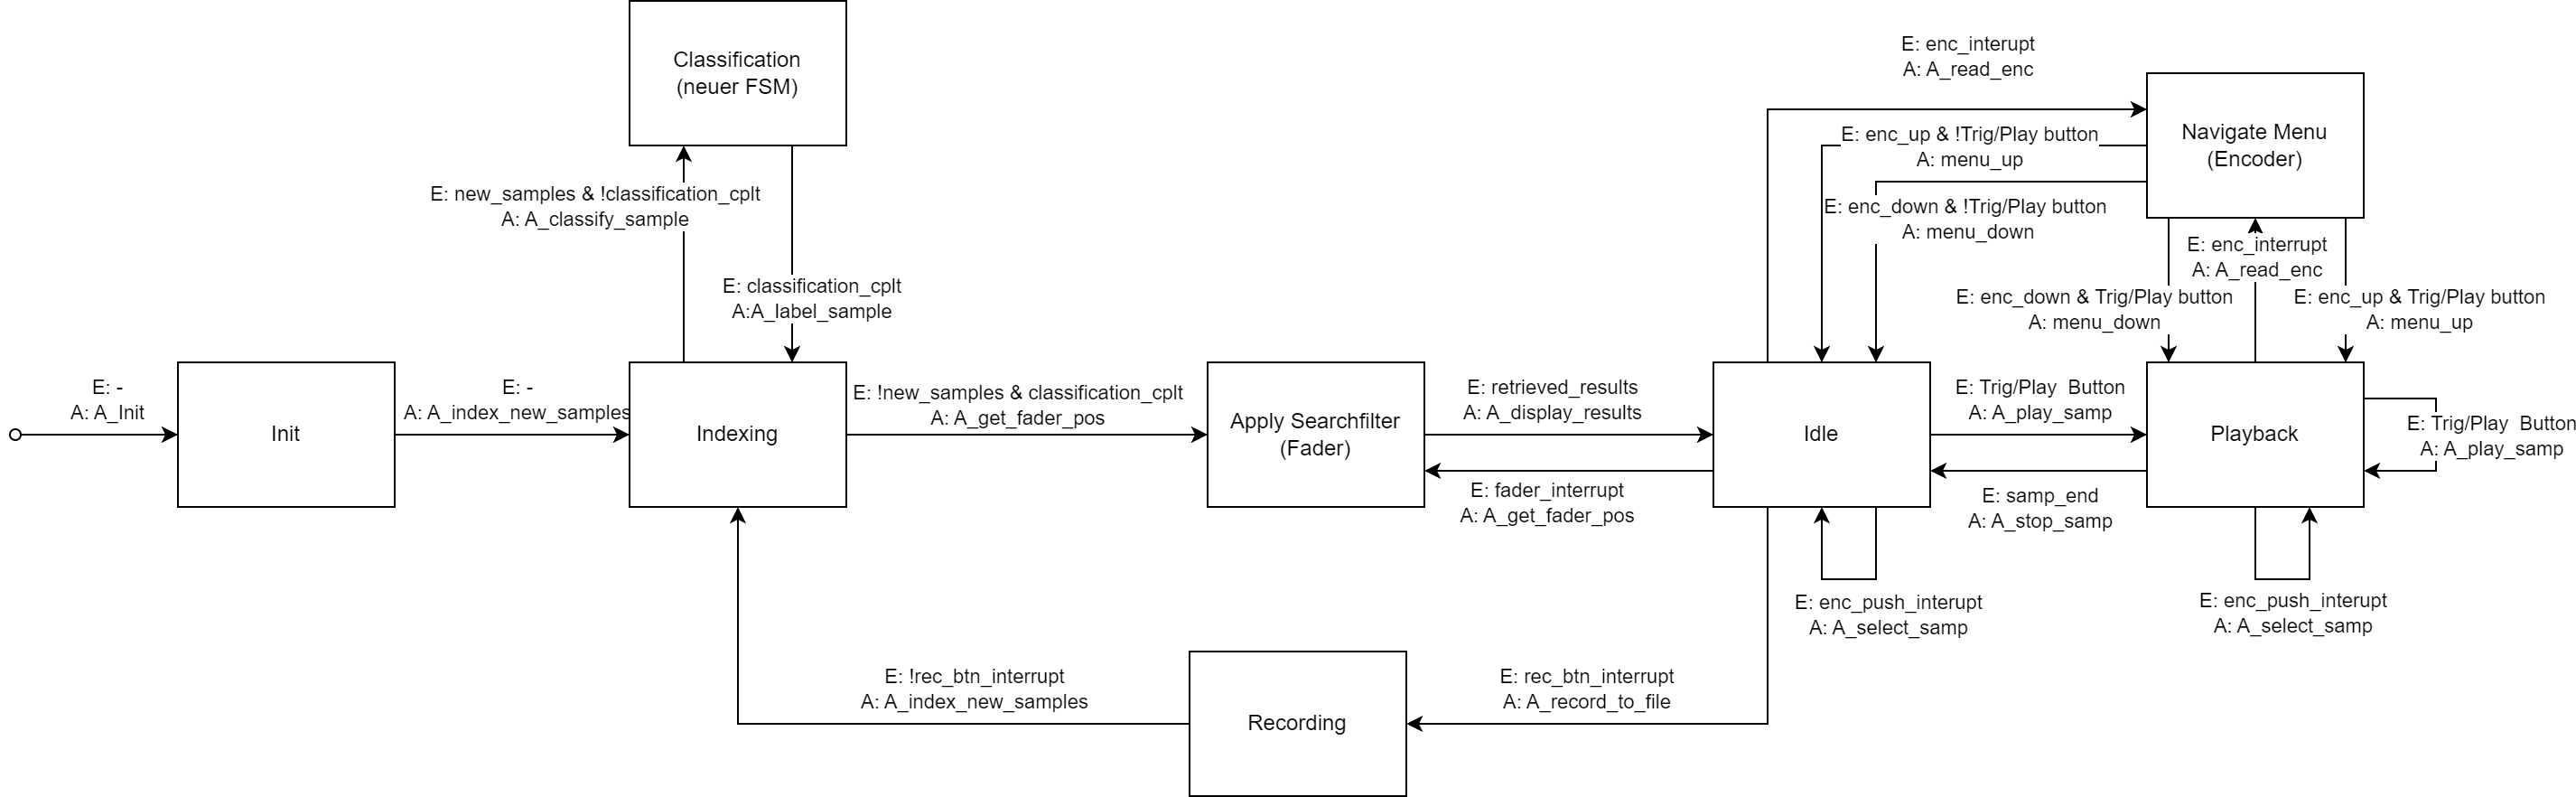
\includegraphics[width=1.0\textwidth]{images/04_spezifikation/fsm.drawio.png}
   	\caption{Zustandsautomat des Systems}
   	\label{fig:fsm}
\end{figure}
% TODO: FORMULIEREN

Nach dem Initialisierungszustand \textbf{Init} beginnt der Automat im \textbf{Indexing}-Zustand. In diesem Zustand wird überprüft, ob noch unklassifizierte Samples vorhanden sind. Falls ja, wechselt der Automat in den \textbf{Classification}-Zustand, um das unklassifizierte Sample zu klassifizieren. 

Nach der Klassifikation kehrt der Automat wieder in den \textbf{Indexing-Zustand} zurück, um zu überprüfen, ob noch weitere unklassifizierte Samples vorhanden sind. Dieser Prozess wiederholt sich, bis alle Samples klassifiziert sind.

Sobald alle Samples klassifiziert sind, wechselt der Automat in den \textbf{Idle-Zustand}. Hier wird der Suchfilter angewendet, der mit fünf Fadern eingestellt ist, und die entsprechenden Samples werden auf dem Display angezeigt. Im \textbf{Idle}-Zustand können die Samples entweder abgespielt (im \textbf{Playback}-Zustand) oder über den \textbf{Navigate Menu}-Zustand durch das Menü navigiert werden.

Wird ein neues Sample (\textbf{Recording}-Zustand) aufgenommen, erfolgt die Klassifikation wie nach Intialisierung des Systems über den \textbf{Indexing-Zustand}.

Nach Änderung der Faderstellung, wird der Suchfilter wieder angewandt (\textbf{Apply-Searchfilter}-Zustand).

\subsection{Arbeitspakete}

    \begin{figure}[H]
	\centering
	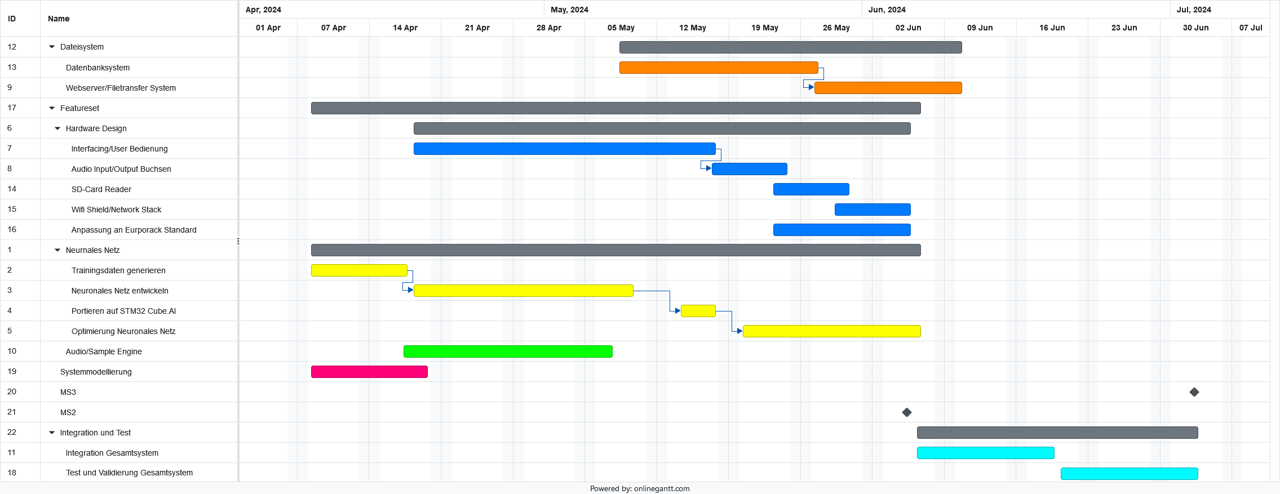
\includegraphics[width=1.0\textwidth]{images/04_spezifikation/gantt.png}
	\caption{GANTT Diagramm}
	\label{fig:gantt}
\end{figure}


Aufgabenaufteilung erläutern